\documentclass[twoside]{article}

\usepackage{amsmath,amsthm,amssymb,graphicx}
\usepackage{hyperref}
\usepackage[numbers]{natbib}
\usepackage{float}
\usepackage{bbm}

\theoremstyle{definition}
\newtheorem{thm}{Theorem}[section]
\newtheorem{lem}[thm]{Lemma}
\newtheorem{prop}[thm]{Proposition}
\newtheorem{cor}[thm]{Corollary}
\newenvironment{pf}{{\noindent\sc Proof. }}{\qed}
\newenvironment{map}{\[\begin{array}{cccc}} {\end{array}\]}

\newcommand{\comment}[1]{}
\theoremstyle{definition}
\newtheorem*{defn}{Definition}
\newtheorem*{exmp}{Example}
\newtheorem*{prob}{Problem}

\theoremstyle{remark}
\newtheorem*{rem}{Remark}
\newtheorem*{note}{Note}
\newtheorem*{exer}{Exercise}

\setlength{\oddsidemargin}{0.25 in}
\setlength{\evensidemargin}{-0.25 in}
\setlength{\topmargin}{-0.6 in}
\setlength{\textwidth}{6.5 in}
\setlength{\textheight}{8.5 in}
\setlength{\headsep}{0.75 in}
\setlength{\parindent}{0 in}
\setlength{\parskip}{0.1 in}

\newcommand{\widgraph}[2]{\includegraphics[keepaspectratio,width=#1]{#2}}
\newcommand{\widgraphr}[3]{\includegraphics[keepaspectratio,width=#1,angle=#3]{#2}}

\newcommand{\lecture}[4]{
   \pagestyle{myheadings}
   \thispagestyle{plain}
   \newpage
   \setcounter{page}{1}
   \noindent
   \begin{center}
   \framebox{
      \vbox{\vspace{2mm}
    \hbox to 6.28in { {\bf Stat365/665 (Spring 2015) Data Mining and Machine Learning \hfill Lecture: #4} }
       \vspace{6mm}
       \hbox to 6.28in { {\Large \hfill #1  \hfill} }
       \vspace{6mm}
       \hbox to 6.28in { {\it Lecturer: #2 \hfill Scribe: #3} }
      \vspace{2mm}}
   }
   \end{center}
   \markboth{#1}{#1}
   \vspace*{4mm}
}


%%%%%%%
% Some commonly used notation
%%%%%%%

\def\R{{\mathbb R}}
\def\X{{\mathcal X}}
\def\Y{{\mathcal Y}}
\def\H{{\mathcal H}}
\def\E{{\mathbb E}}
\def\sign{{\rm sign}}

\newcommand{\percent}{$\%$}

\begin{document}
\textbf{Machine Learning, Homework 3}\\
\textbf{Leon Lixing Yu}\\
In collaboration with: Junaid Nomani, Faisal Zaghloul\\

\section{Boosting and overfitting}
The decision tree I used is matlab function $fitctree$, which takes inputs, $Y$, $X$, $weights$, and $maxNumSplits$. The maximum number of splits are used to control the depth of the tree.\\
If the $maxNumSplits$ is $3$, the depth of the tree is 2. likewise, if the $maxNumSplits$ is $4$, the depth of the tree is 3. Since we are given the depth of the tree as $3$, I choose the $maxNumSplits = 4$. \\
The code for this problem is attached in \textbf{Appendix-A}.The figures below shows the test errors while changing the number of iterations with fixed tree depth.  

\begin{figure}[H]
\centering
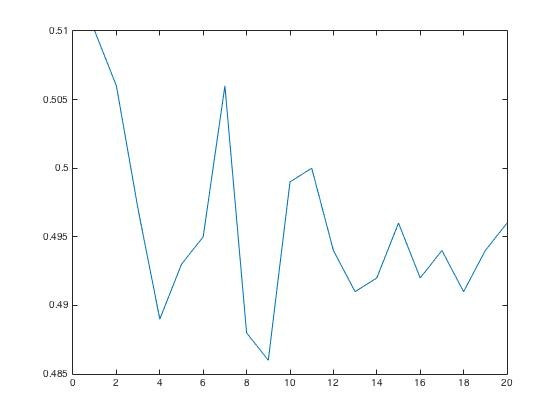
\includegraphics[width=120mm]{problem1_1.jpg}
\caption{test error for up to 200 iterations.I can see a dip at about 30th iteration. The testing error fluctuates alone the similiar domain.It is possible a overfitting case after 30 iterations. To clearify, I plotted training error to see the convergence.}
\end{figure}

\begin{figure}[H]
\centering
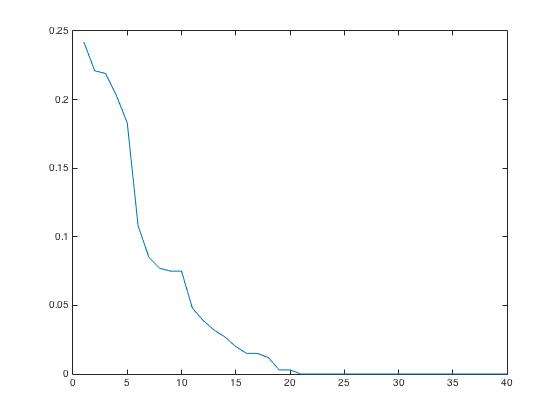
\includegraphics[width=120mm]{problem1_2.jpg}
\caption{training error for up to 200 iterations.I can see at around 30th iteration, The training takes a huge leap, yet the progression on training accuracy slows down afterwards. I suspect that the training is overfitted to the dataset. after 30th iterations.}
\end{figure}

The figure below shows the graph for testing error with incremental tree depth while fixing the iteration number to $3$
\begin{figure}[H]
\centering
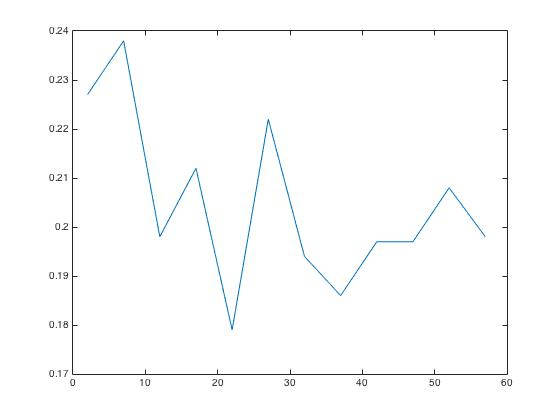
\includegraphics[width=120mm]{problem1_3.jpg}
\caption{Training error for upto $60$ splits. The iteration is fixed to 10. I see that there are a few fluctuation yet the overall error rate is improving slightly }
\end{figure}



\section{boosting for regression}
The algorithm is shown below:
\begin {verbatim} 
The initial residual is set to be the training label, Y. 

for each iteration
    I train a decision tree of depth 3 to fit the residual
    Get the prediction based on trained tree for testing set and training set
    Update F = F + prediction (for testing)
           Ftrain = Ftrain + predictionTrain ( for training)
    Update residual to the error between the prediction and labels for both testing and training sets (residual = y - prediction)

The error is the 2 norm of of the residual after all iterations.
The F in the end of all iterations are the prediction for the testing set
\end{verbatim}

The implementation of the algorithm is shown in \textbf{Appendix-B}. The graph below shows the testing error. 
\begin{figure}[H]
\centering
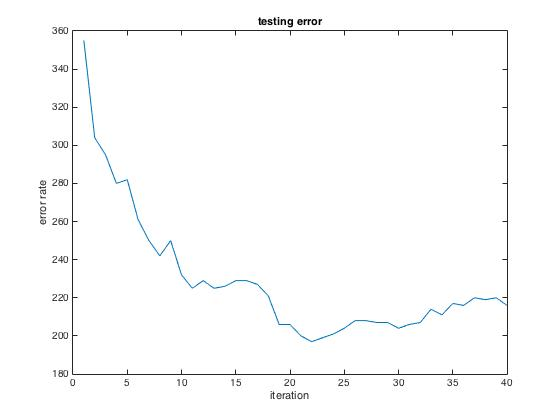
\includegraphics[width=120mm]{problem2_1.jpg}
\caption{test error for upto 50 iterations.I can see the improvement on higher iteration choices, yet at iteration = 10, the performance gain stopped; thus I suspect overfitting if I go beyond 10 iterations. To verify my claim, I also plot the training error. }
\end{figure}

\begin{figure}[H]
\centering
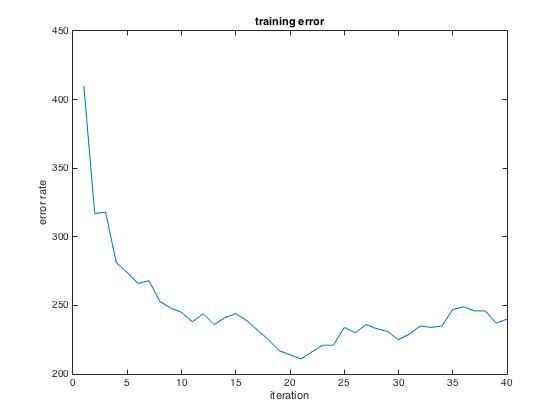
\includegraphics[width=120mm]{problem2_2.jpg}
\caption{training error for upto 50 iterations. I can see the convergence happening, yet since the testing error is hiccupped at iteration = 10, I think the training is overfitted to the training set after 10th iteration. }
\end{figure}

\section{Model Selection}
The code for this section is shown in \textbf{Appendix-C}. I use forward selection for this dataset as when I tried LARS, it did not work as well. The forward selection is working much better. The figure below shows the plot comparsion between real labels and fitted functions 
\begin{figure}[H]
\centering
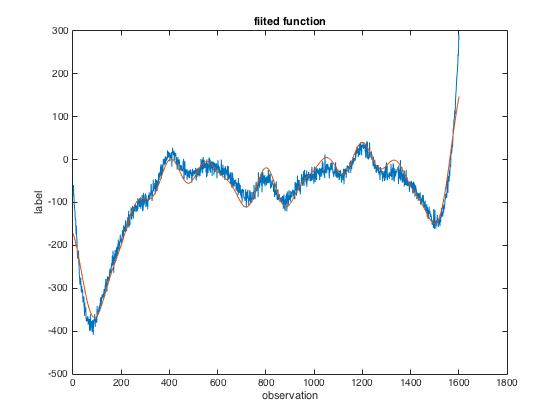
\includegraphics[width=120mm]{problem3_1.jpg}
\caption{The thin curve is fitted linear combination from the forward selection, and the data points are the labels. I see that the fitted function well fits the data points.}
\end{figure}
The fitted results are:\\ 
$\;\;\;\; x^2$ with coeff $2.3543$\\
$\;\;\;\; x^3$ with coeff $0.3120$\\
$\;\;\;\; cos(wx) \;\;\;\; where \; w \in {2\pi i /1000}\;\;\;\; where \;\;\;\; i = {0, 149, 220, 291, 298, 503, 757}$ with respective coeffs $ {-140.0, -141.993, 9.3862, -164.25411, 120.5357, 24.3701, 16.3127}$\\
$\;\;\;\; exp(-x^2/(2\sigma^2)) \;\;\;\; where \sigma \in {i/100} \;\;\;\; where\;\;\;\; i = 88$ with respective coeffs $256.5708$.

\section{term project}
My term project partner is Junaid Nomani. Therefore, my project description would be the same as his. 

Ai for game playing.\\
Partner: Junaid Nomani\\
Our final project is to use machine learning techniques to get an AI to learn how to play 4x4 tic-tac-toe without any user defined features. We hope to use online learning where the AI improves its performance just by playing. As input it sees the current board state, and as output it chooses the position to place its next token. It trains based only on if it won a game or lost a game. It can play against a human to learn, but to make it faster and so we don’t have to play thousands of games of tic-tac-toe we will use hand-coded AI for the learning AI to play against. \\
We hope to try a few algorithms to see which work best, but will probably prefer using feed-forward neural networks and maybe SVMs. We will test the AIs performance by looking at it’s winrate against the hand-coded AI for recent games it has played.\\ 





\end{document}
